\subsection{Matching Pennies}

\subsubsection{Descripción del Juego}

En este juego cada jugador tiene una moneda y selecciona cara o sello de forma secreta. Si las elecciones son gana el jugador $1$, en caso contrario gana el jugador $2$. La matriz de pagos de este juego se muestra en la Tabla \ref{table:pagos-matching-pennies}
\begin{table}[ht]
\begin{center}
\caption[Tabla de pagos del juego matching pennies]{Tabla de pagos del juego \textit{matching pennies}}
\label{table:pagos-matching-pennies}
\begin{tabular}{ c | c | c |}
 & cara & sello  \\ \hline
 cara  &  1 & -1 \\ \hline
 sello & -1 &  1 \\ \hline
\end{tabular}
\end{center}
\end{table}

El problema de programación lineal asociado es el siguiente
\begin{equation}
\begin{array}{r r r r r r r r}
\max  & z &  & & & & &\\
\text{s.a.}  
&   &   & x_1  & + & x_2 & = & 1 \\
& z & - & x_1  & + & x_2 & \leq & 0 \\
& z & + & x_1  & - & x_2 & \leq & 0 \\
&   &   & x_1, &   & x_2 & \geq & 0
\end{array}
\end{equation}
Cuya solución primal viene dada por $(z*, x_1^*, x_2^*) = (0, \frac{1}{2}, \frac{1}{2})$ y su solución dual por $(w^*, y^*_1, y^*_2) = (0, \frac{1}{2}, \frac{1}{2})$. Luego el equilibrio de Nash se obtiene cuando ambos jugadores eligen cara o sello con probabilidad $\frac{1}{2}$ y el valor del juego es igual a $0$.

\subsubsection{Resultados experimentales}

En este juego, si un jugador elige cada acción con una probabilidad de $0.5$, entonces su ganancia esperada es igual a $0$, sin importar la estrategia de su oponente, obteniendo el equilibrio de Nash cuando ambos jugadores utilizan esta estragia. Las estrategias obtenidas no corresponden al equilibrio de Nash, sin embargo, garantizan una utilidad cercana a $0$ en todos los casos, siendo la más baja igual a $-0.008$, como se muestra en la Tabla \ref{tab:estrategias-matching-pennies}. Por lo que todas las estrategias obtenidas son un $\varepsilon$- equilibrio de Nash, con $\varepsilon < 0.008$.

\begin{table}[hbt!]
    \centering
    \begin{tabular}{c|c|c|c|c}
        & E.N. & A & B & C \\ \hline
        $\sigma_1$   & $(0.500, 0.500)$ & $(0.500, 0.500)$ & $(0.500, 0.500)$ & $(0.500,  0.500)$ \\
        $\sigma_2$   & $(0.500, 0.500)$ & $(0.497, 0.503)$ & $(0.503, 0.497)$ & $(0.504,  0.496)$ \\ \hline
        $(v_1, v_2)$ & $(0.000, 0.000)$ & $(0.000, -0.006)$ & $(0.000, -0.006)$ & $(0.000, -0.008)$ \\ \hline
    \end{tabular}
    \caption{Estrategias obtenidas del juego Matching Pennies}
    \label{tab:estrategias-matching-pennies}
\end{table}


La Tabla \ref{tab:resultados-matching-pennies} muestra los resultados obtenidos relacionados al tiempo y número de iteraciones de los procedimientos. El procedimiento A, regret condicional, tuvo una duración promedio de $10.276$ segundos, con un número promedio de iteraciones de $3892550.4$, obteniendo un promedio de $2.64 {\times} 10^{-6}$ segundos por iteración. Con el procedimiento B, que utiliza un vector invariante de probabilidad, se obtuvo un tiempo, número de iteraciones y tiempo por iteración promedios de $3.777$ segundos, $25616.6$ iteraciones y $3.03 {\times} 10^{-5}$ segundos por iteración, respectivamente. Por último, el procedimiento C, regret incondicional, se obtuvo un tiempo promedio de $0.042$, el número de iteraciones promedio fue de $16260.5$, obteniendo un promedio de $2.58 {\times} 10^{-6}$ segundos por iteración. 

\begin{table}[hbt!]
\scriptsize
    \centering
    \begin{tabular}{r r r | r r r | r r r}
    \multicolumn{3}{c}{A} & \multicolumn{3}{c}{B} & \multicolumn{3}{c}{C} \\ \hline
    $T$ & $I$ & $T/I$ & $T$ & $I$ & $T/I$ & $T$ & $I$ & $T/I$ \\  \hline
	$7.663$ & $3068341$ & $2.50 {\times} 10^{-06}$ & $0.985$ & $32510$ & $3.03 {\times} 10^{-05}$ & $0.002$ & $955$ & $2.53 {\times} 10^{-06}$ \\
	$9.650$ & $3857071$ & $2.50 {\times} 10^{-06}$ & $1.748$ & $56946$ & $3.07 {\times} 10^{-05}$ & $0.064$ & $24968$ & $2.55 {\times} 10^{-06}$ \\
	$23.313$ & $8950013$ & $2.60 {\times} 10^{-06}$ & $0.552$ & $18401$ & $3.00 {\times} 10^{-05}$ & $0.061$ & $23854$ & $2.57 {\times} 10^{-06}$ \\
	$11.757$ & $4240611$ & $2.77 {\times} 10^{-06}$ & $0.309$ & $10197$ & $3.03 {\times} 10^{-05}$ & $0.025$ & $9724$ & $2.57 {\times} 10^{-06}$ \\
	$2.377$ & $877335$ & $2.71 {\times} 10^{-06}$ & $0.747$ & $24892$ & $3.00 {\times} 10^{-05}$ & $0.011$ & $4188$ & $2.59 {\times} 10^{-06}$ \\
	$5.062$ & $1818992$ & $2.78 {\times} 10^{-06}$ & $0.848$ & $28142$ & $3.01 {\times} 10^{-05}$ & $0.025$ & $9666$ & $2.60 {\times} 10^{-06}$ \\
	$4.281$ & $1557496$ & $2.75 {\times} 10^{-06}$ & $0.132$ & $4405$ & $3.01 {\times} 10^{-05}$ & $0.045$ & $16951$ & $2.64 {\times} 10^{-06}$ \\
	$22.110$ & $8230100$ & $2.69 {\times} 10^{-06}$ & $1.307$ & $43116$ & $3.03 {\times} 10^{-05}$ & $0.021$ & $8155$ & $2.64 {\times} 10^{-06}$ \\
	$3.691$ & $1432846$ & $2.58 {\times} 10^{-06}$ & $0.639$ & $21311$ & $3.00 {\times} 10^{-05}$ & $0.093$ & $35270$ & $2.64 {\times} 10^{-06}$ \\
	$12.853$ & $4892699$ & $2.63 {\times} 10^{-06}$ & $0.500$ & $16246$ & $3.08 {\times} 10^{-05}$ & $0.076$ & $28874$ & $2.64 {\times} 10^{-06}$ \\ \hline
	$10.276$ & $3892550.4$ & $2.64 {\times} 10^{-06}$ & $0.777$ & $25616.6$ & $3.03 {\times} 10^{-05}$ & $0.042$ & $16260.5$ & $2.58 {\times} 10^{-06}$ \\ \hline
    \end{tabular}
    \caption{Resultados del juego Matching Pennies}
    \label{tab:resultados-matching-pennies}
\end{table}

La Figura \ref{fig:regret-matching-pennies} muestra el regret incondicional con respecto al tiempo de la última corrida, para los $3$ procedimientos. Se observa que en todos los casos el \textit{regret} total de cada jugador converge a cero.

\begin{figure}[hbt!]
\caption{Gráficas del regret con respecto al número de iteraciones del juego Matching Pennies}
\label{fig:regret-matching-pennies}
\centering
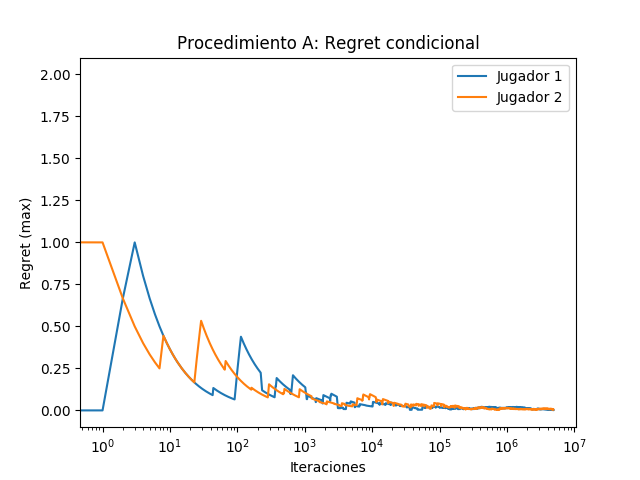
\includegraphics[width=0.45\textwidth]{graficas/matching-pennies/procedimiento-A.png}
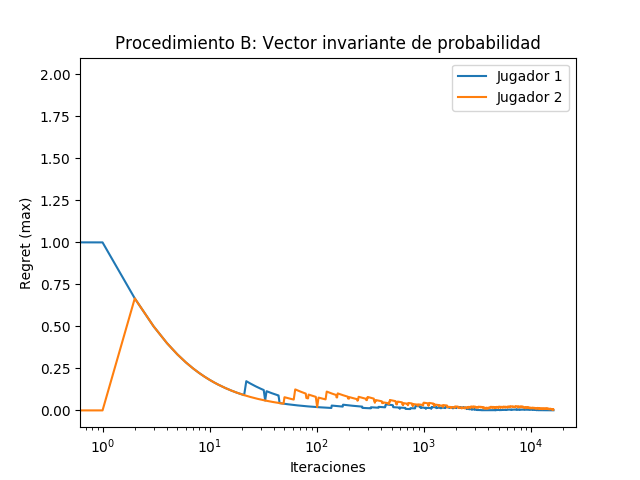
\includegraphics[width=0.45\textwidth]{graficas/matching-pennies/procedimiento-B.png}
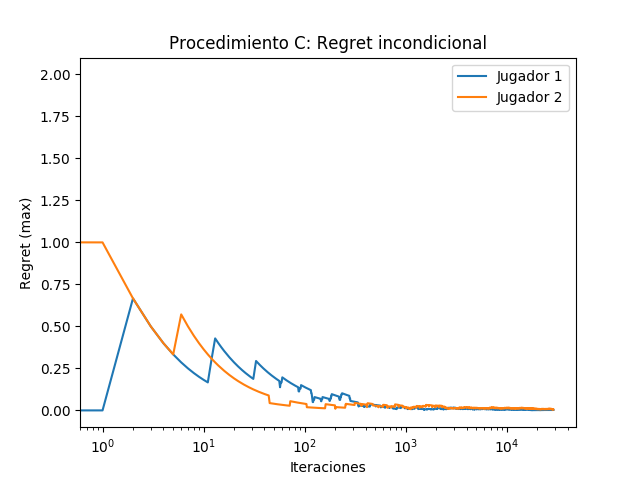
\includegraphics[width=0.45\textwidth]{graficas/matching-pennies/procedimiento-C.png}
\end{figure}
